%!TEX root = ../username.tex
\chapter[Theory]{Theory}\label{chapter:theory}

\section{Waveforms}\label{section:waveforms}
According to Joseph Fourier, the creator of the Fourier Transform, any periodic signal or sound can be reduced into their individual sine waves, or other waveform types \cite{Broughton_Bryan_2008}. There are five basic waveform types: a sine wave, square wave, sawtooth wave, triangle wave, and pulse wave \cite{Winer_2018}. The pulse wave is a special type of waveform, as it is a non-sinusoidal waveform which includes square waves within it, and is similarly periodic to square waves, but also asymmetrical. The other waveform types are also periodic waves, as they repeat in a pattern of motion known as a cycle, and the period is the time length.

The speed with which each wave rises and falls is its frequency. If the frequency is too low (less than 20 cycles per second, or 20 Hertz, abbreviated as Hz), little to no noise will be audible by the human ear. If the frequency is too high (generally above 20,000 cycles per second, or 20 kiloHertz, abbreviated kHz), again, few noises besides high-pitched and shrill noises will be audible. The range of human hearing is generally stated as being from 20 cycles per second, with 20 Hertz at the low end to 20,000 cycles per second (20 kHz) at the high end. Older people generally lose the ability to hear the higher frequencies.

\begin{figure}
	\centering
	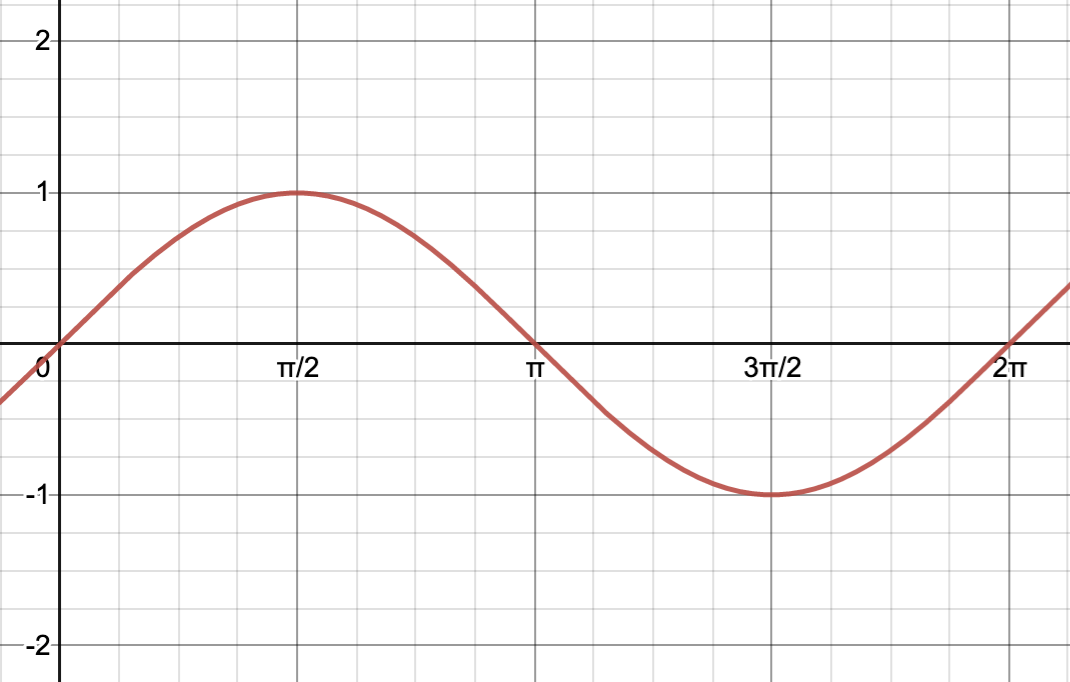
\includegraphics[width=0.5\textwidth]{figures/sine-wave-form.png}
	\caption{A basic sine wave}
	\label{fig:basic-sine-wave}
\end{figure}

\subsection{Sine Waves}\label{subsection:sine-waves}
The first of the basic periodic waves is the sine wave, and is the most common type of periodic wave. The sine wave is a signal with only one frequency, and represents the unidimensional motion for any signal with a phase angle that rotates at a constant rate. It is also based on the trigonometric sine function. On the unit circle, the trigonometric sine function of a phase angle $\theta$ is defined as the ratio of the length of the opposite side and the hypotenuse of a right triangle. The unit circle, with a radius of 1, results in the sine function $sin\theta$ being equal to the y-value in Cartesian coordinates, where the hypotenuse of the right triangle that is formed meets the circle, like in Figure \ref{fig:unit-circle}. We can then use this trigonometric sine wave to synthesize a sine wave audio signal. As sine wave is a continuous periodic wave, in which the wave continues to sound until stopped, we must use the sine wave function on the unit circle continuously. Thus, we use the sine function continuously around the unit circle, going counterclockwise. We notice that in the correlation between Figures \ref{fig:basic-sine-wave} and \ref{fig:unit-circle} moving counterclockwise through the unit circle results in the appropriate rise and fall of the sine wave. $\frac{\pi}{2}$ is the highest y-value within the Cartesian plane, and so denotes a peak in the sine wave, while $\frac{3\pi}{2}$ is the lowest, denoting a trough.

\begin{equation}
	y = Asin(B(x + C)) + D
	\label{eq:sine-wave-equation}
\end{equation}

Like with the other periodic waves, sine waves have three important properties: frequency, amplitude, and phase. From the generic function for a sine wave as in Equation \ref{eq:sine-wave-equation}, we are able to compute the various properties. First, \textit{A} is the sine wave's amplitude. This is defined as the height from the center line of the wave to its peak or trough. For our unit sine wave, this value will be 1. Second is the variable \textit{B}, which helps to define the period of the wave, or the distance between one peak and the next, or one trough and the next. With Equation \ref{eq:sine-wave-period}, we see the period is equivalent to taking the total circumference of the unit circle, and dividing it by \textit{B}. Third, the phase shift of a sine wave is denoted by \textit{C}. If the expression is $(x + C)$, then the phase of the sine wave will shift to the left, as the x-value of the wave becomes negative \textit{C}. Otherwise, if the expression is $(x - C)$, then the wave will shift right, with a positive x-value as \textit{C}. Finally, the variable \textit{D} is equivalent to the vertical shift of the wave. This notates the distance that the wave will shift vertically from its unit circle position.

\begin{equation}
	\frac{2\pi}{B}
	\label{eq:sine-wave-period}
\end{equation}

\begin{figure}
	\centering
	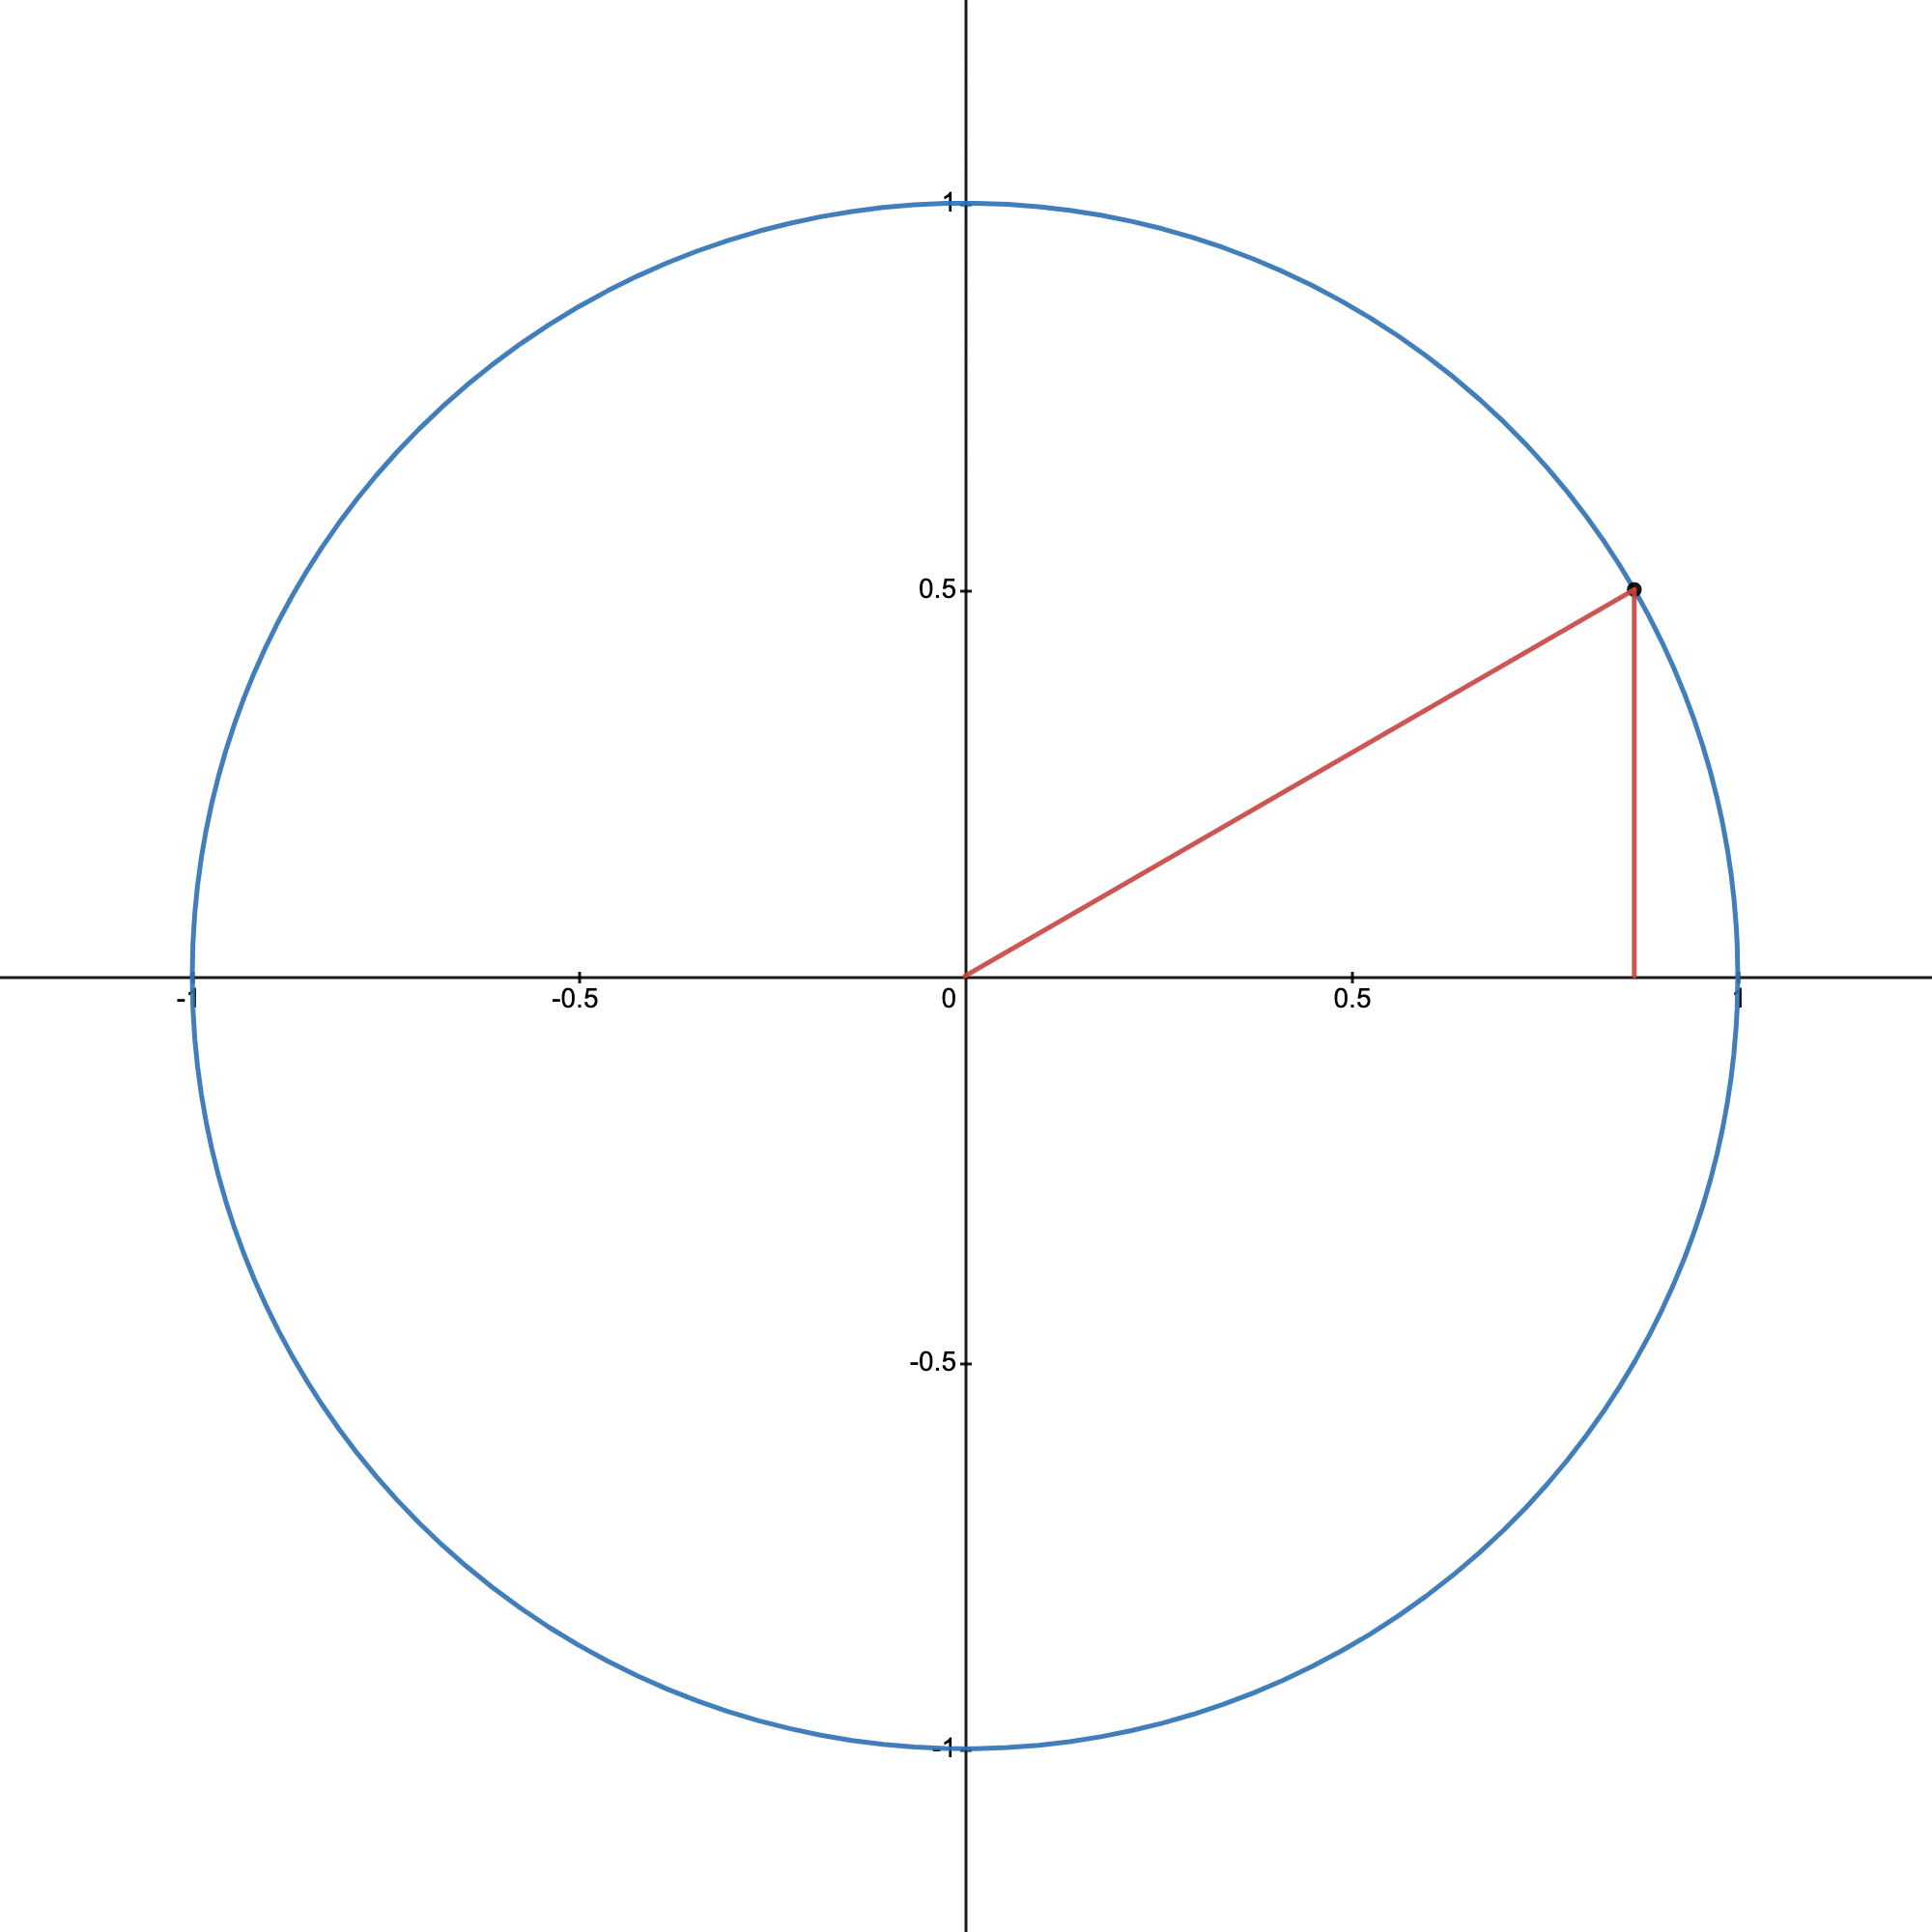
\includegraphics[width=0.5\textwidth]{figures/unit-circle.png}
	\caption{The unit circle}
	\label{fig:unit-circle}
\end{figure}

\subsection{Square Waves}
The square wave is the second of the periodic waveforms, and is a wave in which the frequency oscillates between a single fixed minimum and maximum value \cite{Tarr_2019}. Within the unit circle definition of the square wave, the maximum frequency is positive or negative one, as in Figure \ref{fig:square-wave}. This unit square wave details the ideal square wave, in which the change between minimum and maximum frequency happen instantaneously. An approximation of square waves may be created through the combination of multiple individual harmonics (sine functions). This method of creating an audio signal is known as \textit{additive synthesis}, in which a new timbre or sound is create by adding together periodic waveforms, usually sine waves \cite{Tarr_2019}. 

The square wave is a certain type of pulse wave (discussed separately in section \ref{subsection:pulse-wave}) which allows for a frequency to sound at fixed amplitudes for an arbitrary duration. At its simplest, a square wave can be defined as a sign function of a sinusoidal. A sign function, or a signum function, as in Figure \ref{fig:sign-function}, is an odd mathematical function which extracts the sign of a real number, expressed as $sgn$. Of a real number $x$, it is a piecewise function, defined as in Equation \ref{eq:sgn-function}.

\begin{equation}
	sgn (x): \begin{cases}
		-1 & \textrm{if } x < 0, \\
		0 & \textrm{if } x = 0, \\
		1 & \textrm{if } x > 0
	\end{cases}
	\label{eq:sgn-function}
\end{equation}

\begin{figure}
  \centering
  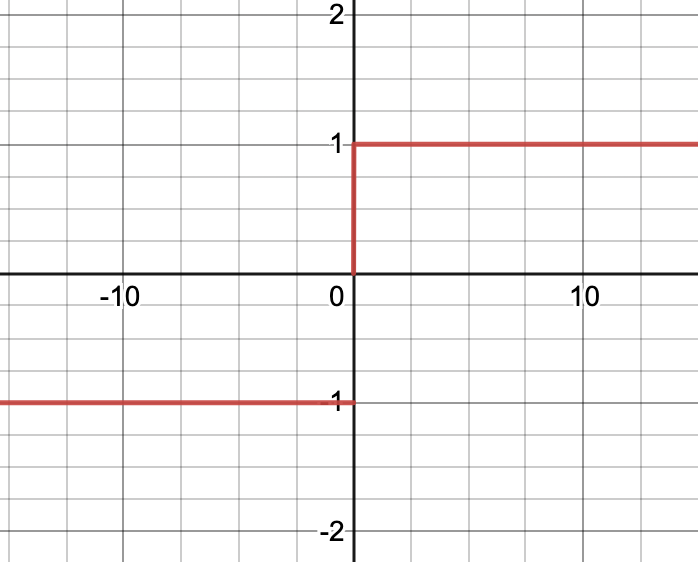
\includegraphics[width=0.5\textwidth]{sign-function.png}
  \caption{A sign function}
  \label{fig:sign-function}
\end{figure}

Thus, we have a square wave equal to Equation \ref{eq:square-wave-function}. The function $x(t)$ will equal 1 when the sinusoidal is positive, -1 when negative, and 0 at the discrete values where the sinusoidal is equivalent to 0.

\begin{align}
	x(t) = sgn(sin(\frac{2\pi\textrm{t}}{T}) &
	= sgn(sin2\pi ft)
	\label{eq:square-wave-function}
\end{align} %TODO: write out periodic function to compare with sawtooth


\begin{figure}
  \centering
  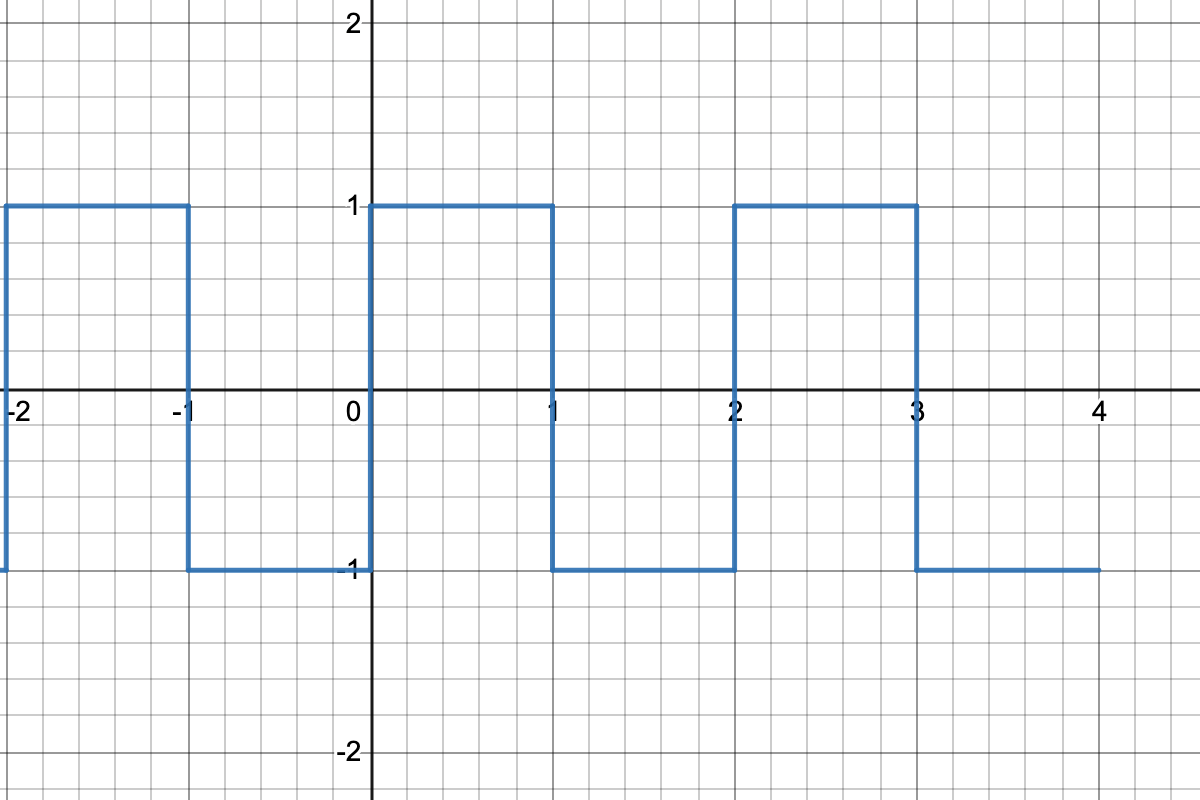
\includegraphics[width=0.5\textwidth]{figures/square-wave.png}
  \caption{A basic square wave}
  \label{fig:square-wave}
\end{figure}

\subsection{Sawtooth Waves}
The sawtooth waveform is also a non-sinusoidal wave, which resembles the teeth of a plain-toothed saw. Similar to the square wave, a sawtooth wave will ramp upwards to a peak amplitude height, then sharply drop to its trough, as in Figure \ref{fig:basic-sawtooth-wave}. Then, we are able to take Equation \ref{eq:sawtooth-piecewise-function}, and place it into a periodic function, as in Equation \ref{eq:sawtooth-sinusoidal-function}. For the periodic function, let $frac(x) = t - \lfloor t \rfloor$.

\begin{equation}
	x(t) = t - \lfloor t \rfloor
	\label{eq:sawtooth-piecewise-function}
\end{equation}

\begin{equation}
	S(x) = Afrac(\frac{x}{T} + \phi)
	\label{eq:sawtooth-sinusoidal-function}
\end{equation}

Like with other waveforms, the variable \textit{A} represents the wave's amplitude, and \textit{T} represents the wave's period. The variable $\phi$ denotes the wave's phase, with positive values causing a shift to the left, and negative values a shift to the right. Sawtooth waves are typically created through additive synthesis, much like square waves are, and so we notice that sawtooth waves and square waves have similar periodic equations \cite{Tarr_2019}.

\begin{figure}
  \centering
  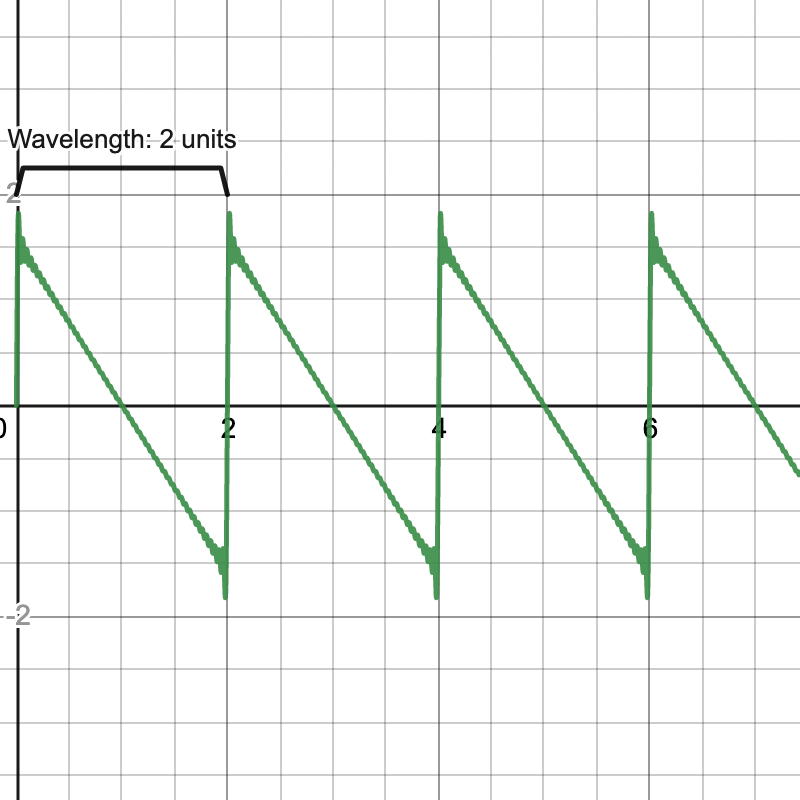
\includegraphics[width=0.5\textwidth]{figures/sawtooth-wave.png}
  \caption{A basic sawtooth wave}
  \label{fig:basic-sawtooth-wave}
\end{figure}


\subsection{Triangle Wave}

A triangle wave is also a non-sinusoidal waveform, named for its triangular shape. Like with square waves, this type of wave only contains odd harmonics, i.e. only containing valid values which are odd numbers.

\begin{equation}
	f(x) = \frac{2}{\pi}sin^{-1}\lceil sin(\pi x) \rceil
	\label{eq:triangle-wave-function}	
\end{equation}


\subsection{Pulse Wave}\label{subsection:pulse-wave}
The final common waveform type is the pulse wave. This is a non-sinusoidal waveform which includes squares waves, in which the shape of the wave is determined by the pulse width of the input. However, unlike with square waves, the second half of a cycle within a pulse wave is replaced with silence, as in Figure %TODO: insert figure of pulse wave.

\section{Time Domain and Frequency Domain}

Digital signals are studied in one of four domains: time domain, spatial domain, frequency domain, and wavelet domain. For the purposes of this research, we focus most on only two of these domains: the time domain and the frequency domain. These domains are most commonly used in audio analysis and synthesis. Digital audio is normally viewed in the time domain, and through the use of the Discrete Fourier Transform (sometimes also called the Fast Fourier Transform), we are able to produce a frequency domain representation for frequency analysis.

\subsection{Time Domain}

Audio is most commonly represented as a waveform, most commonly as the sine wave, with time plotted against the wave's amplitude. The x-axis will represent the discrete audio signal, and is normalized to represent the hours, minutes, or seconds. Normalization is the process of transposing a data set to a specific reference value, by dividing the output value by a given constant \cite{Zjalic_2021}. In audio, the most common type of normalization will be applied to a common audio waveform, to produce a signal that is normalized between the values of 1 and -1. 1 thus becomes the reference value for positive values, and -1 for negative values. To normalize audio, the following formula is applied to an audio signal: sample value $\times$ $\frac{1}{\textrm{reference value }}$. Audio normalization is useful for audio analysis, in that it allows for comparisons to be made between signals, regardless of their magnitude and sample rate. The y-axis then represents the magnitude of each audio sample, in which the decibels (or another magnitude unit) are a bipolar normalized value, between a positive and negative value. 

To transform the time representation from samples to seconds, the sample rate must first be known. From there, it is simple to transpose \cite{Zjalic_2021}. For example, we assume that for the 44100 samples we have that the sample rate is also 44100 Hz. So, $44100 / 441100 = 1$ second, in that we divide the number of samples by the sample rate, to obtain a time representation in seconds. Another example may showcase this better. Assume we have 2646000 samples, and a sample rate of 44100 Hz. Then, we have $2646000/44100 = 60$ seconds.

\subsection{Frequency Domain}
The physical concept of frequency is relatively simple: it is the number of occurrences per unit of time in a given phenomenon \cite{Gabrielli_2020}. In audio, this becomes the number of repetitions, or cycles, of a sine wave. This type of frequency is known as the \textit{temporal frequency}, and will be denoted with the letter \textit{f}. For acoustic audio signals, we will be describing frequency in Hertz (H).\footnote{The reciprocal of the temporal frequency is known as the period, denoted as capital \textit{T}. This is defined as the time required to completed one full cycle at any given frequency, otherwise known as $T = \frac{1}{\textit{f}}$.} In digital signal processing, we instead will be using angular frequency (radians per second, denoted with $\omega$), which measures the angular displacement per unit of time. Thus, we have the following relation between temporal frequency, angular frequency, and period \cite{Gabrielli_2020}.

\begin{align}
    f &= \frac{\omega}{2\pi} &w &= 2\pi &f &= \frac{2\pi}{T}
\end{align}

To convert a signal into the frequency domain, and to obtain its frequency components, the Fourier Transform can be used\footnote{The Inverse Fourier Transform can be used to go from the frequency domain to the time domain.}. Transforms like these are common in audio signal processing. These are mathematical operations which allow you to observe a signal from a different perspective\footnote{The result of a transform on an audio signal can be seen in figure 2.9 of Gabrielli.}.

\section{Digital Signal Processing (DSP)}

\section{Audio Manipulations}
As previously mentioned in Section \ref{section:modular-synth-what-is}, modular synthesis involves sending an audio signal through patches or modules in a linear format to achieve the desired sound output changes. To explain how these changes occur to a sound wave, we begin with a simple sine wave, as in Figure \ref{fig:sine-wave-period-amplitude}. Sine waves are a waveform which is a function of time \texttt{t}:

\begin{figure}
	\centering
	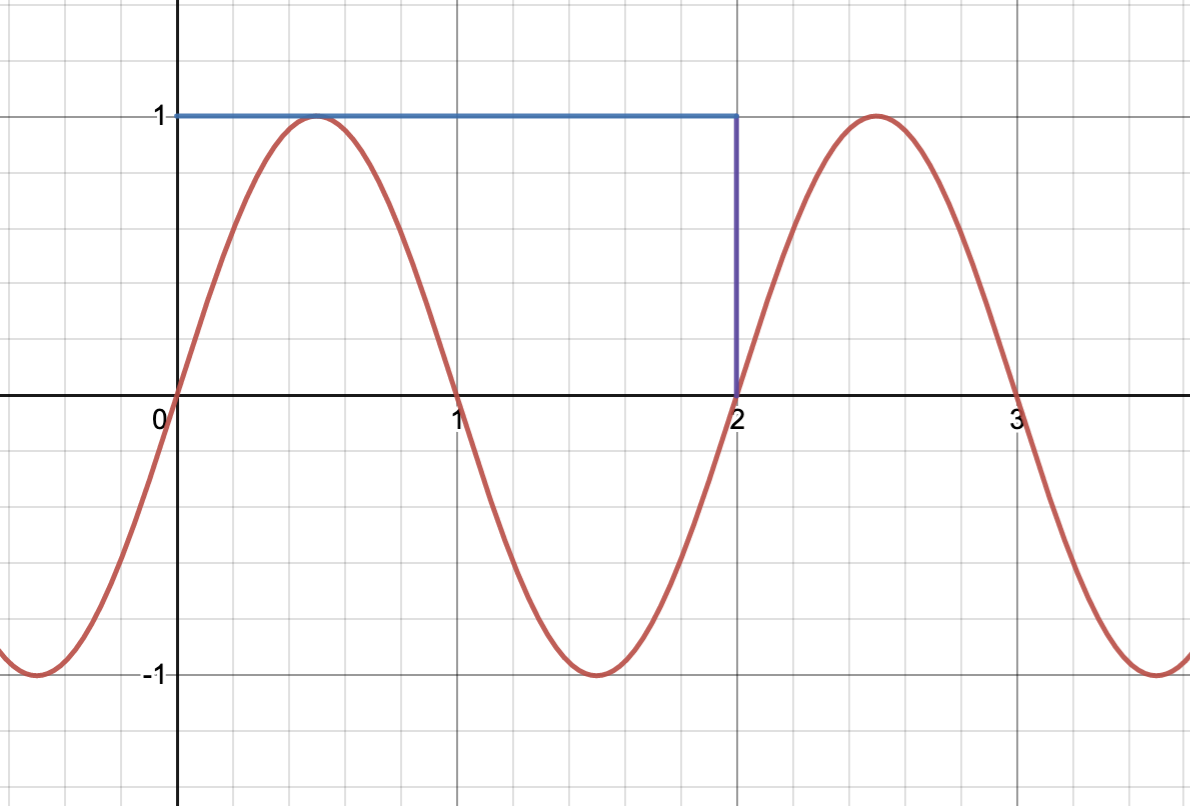
\includegraphics[width=0.5\textwidth]{figures/sine-wave-period-amplitude.png}
	\caption{A basic sine wave, with period demarcated in blue, and amplitude in purple}
	\label{fig:sine-wave-period-amplitude}
\end{figure}

\begin{equation}\label{eq:full-sine-wave-equation}
	y(t) = A \sin(2\pi ft + \varphi) = A\sin(\omega t + \varphi)
\end{equation}

with variables $A$, $f$, $\omega$, $\varphi$. $A$ is the wave's amplitude, which determines the peak deviation from zero. $f$ is the temporal frequency. $w = 2\pi f$ and is the angular frequency, and $\varphi$ is the wave's phase, which specifies (in radians) where in its cycle the wave's oscillation is at time $t$ \cite{Kirk_Hunt_2013}. When $\varphi$ is not equal to zero, the wave itself will appear to be shifted by the value equal to $\varphi / \omega$, which is known as a wave's \say{phase shift.} A negative value will represent a delay in sound, while a positive value will represent an advance in the heard sound.

Thus, there are three primary options when manipulating audio (or a simple waveform); amplitude, frequency, and phase can all be modified at various points to affect the audio output. The first, amplitude, will determine the volume of the wave's sound. The larger the distance between zero and the wave's peak, the louder the human ear will perceive the sound to be\cite{Zjalic_2021}. In Figure \ref{fig:sine-wave-period-amplitude}, amplitude is colored purple, and we see it has a value of 1 (the default value of amplitude of a sine wave from the unit circle), as $A$ does in Equation \ref{eq:full-sine-wave-equation}. By changing the value of $A$ to either $\frac{1}{2}$, or $2$, the peak of the wave will change accordingly, becoming larger or smaller depending on the set value of $A$. This change is reflected in the sound we can hear, as like in Figure \ref{fig:half-sized-sine-wave} and Equation \ref{eq:half-sized-sine-wave}, the volume of this sine wave is halved.

\begin{equation}\label{eq:half-sized-sine-wave}
	y(t) = \frac{1}{2} \sin(\omega t + \varphi)
\end{equation}

\begin{figure}
	\centering
	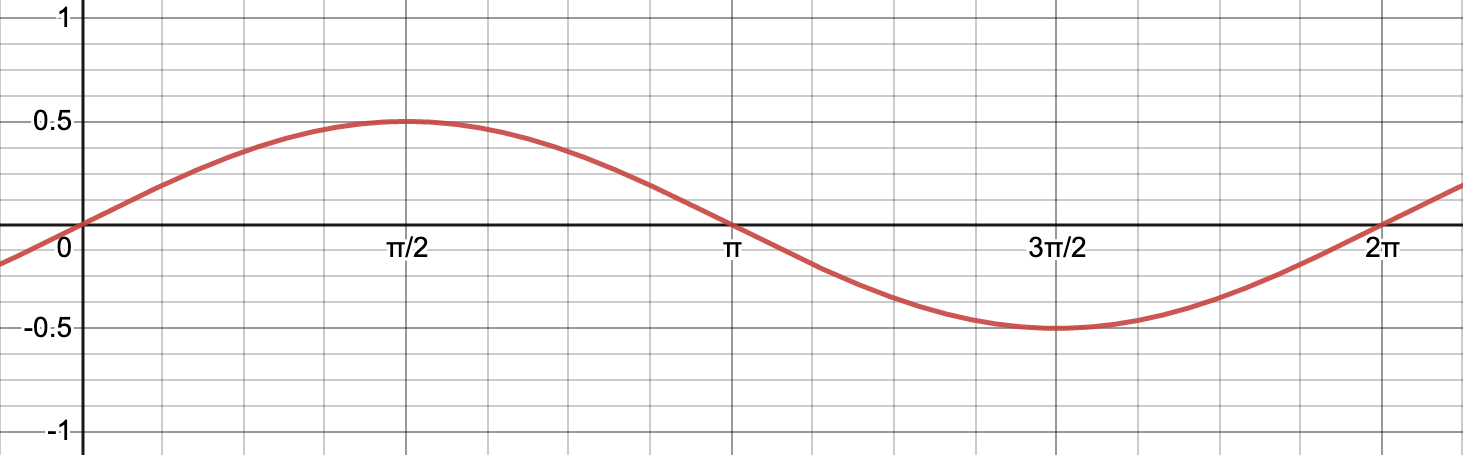
\includegraphics[width=\textwidth]{figures/half-sized-sine-wave.png}
	\caption{A sine wave, with an amplitude of $\frac{1}{2}$}
	\label{fig:half-sized-sine-wave}
\end{figure}

The second option commonly used to manipulate audio is to change an audio signal or wave's temporal frequency. For sound and audio manipulations, the temporal frequency component determines a sound's \say{color,} or \say{timbre.} It is the property of a waveform which determines the output sound's pitch. The high-end of audible frequencies for the human ear is around 20,000 Hz (20 kHz), though this reduces with age. The generally accepted range of human hearing ranges from 20 Hz to 20 kHz, with frequencies below 20 Hz felt more than heard\cite{Rosen_Howell_2011}. This range is further broken down in Table \ref{tbl:frequency-table-of-human-hearing-general}. Thus, with Equation \ref{eq:full-sine-wave-equation}, we change the value of $f$, which will alter the frequency of the wave, and then also alter the perceived pitch. With an increase in temporal frequency, there will also be an increase in angular frequency $\omega$, which increases the rate of change of the sine wave. With the period of the sine wave in Figure \ref{fig:sine-wave-period-amplitude} marked blue, it is this blue section that will increase with an increase in $\omega$. As $\omega$ increases, there are more repetitions of the sine wave's phase, so the audio output's pitch will increase.

\begin{table}
	\begin{tabular}{|p{20em} | p{25em}|}
		\hline
		General Frequency Range & Description of Range \\ 
		\hline
		<20Hz - 60Hz & The lowest threshold of human hearing. This includes many frequencies that are felt and not heard, and provides the \say{rumble} feeling in music. This range gives much of music its power, and is typically known as \say{sub-bass}. \\
		\hline
		60Hz - 250Hz & This range determines the amount of \say{warmth} and how full the sound is perceived to be. The notes fundamental to rhythm lives in this range, and too much sound in this frequency range will result in the overall sound being \say{boomy}, or muddy-sounding and messy. It is otherwise known as the the \say{bass} frequency. \\
		\hline
		250Hz - 500Hz & The lower harmonics of many instruments are in this range. It is generally known as the \say{lower midrange} of frequencies, and can introduce listening fatigue and a telephone-quality to the sound if this range is emphasized too much. \\
		\hline
		500Hz - 2 kHz & This range is considered the middle of the midrange. It gives many instruments prominence in a mix, and determines how audible one instrument or vocalist is in comparison to another. If this range is emphasized, audio output may sound tinny and small, which could lead to listening and ear fatigue, as the human ear is sensitive to the human voice, and the frequencies it covers. \\
		\hline
		2 kHz - 4 kHz & The \say{upper midrange} is responsible for much of the attack sounds on percussive and rhythmic instruments. This range may add presence to the mix if boosted, but if it is emphasized too much, it may mask some speech recognition sounds. Listening fatigue may also set in if this range is emphasized too much, as the slightest boost in this range will result in a noticeable change in the sound's timbre. \\
		\hline
		4 kHz - 6 kHz & This range is known as the \say{presence} range. It defines a sound's clarity and the definition of voices and instruments that are present. If this range is boosted, instruments and voices may sound physically closer to the listener, and vice versa, with reducing this range causing instruments and voices to sound further away. However, if this range is emphasized too much, a harsh, irritating sound may occur. \\
		\hline
		6 kHz - 20 kHz & This range controls the \say{brilliance} and clarity of sounds within the mix. Instead of pitches, this range is composed entirely of harmonics, and brings \say{sparkle} to the sound. This range also may easily cause ear fatigue, as an over-emphasis can increase the hiss heard, and produce sibilance, or an unpleasant tonal harnshness which can happen with consonant syllables (most noticeably: S, T, and Z), especially on vocals. \\
		\hline
	\end{tabular}
\caption[A description of the human hearing range]{Descriptions of general frequencies ranges within the range of human hearing}
\label{tbl:frequency-table-of-human-hearing-general}\cite{Suits_1998}\cite{Zjalic_2021}
\end{table}

Finally, a modification to a wave's phase will determine if the audio signal output is on-time, delayed, or early. The numeric value of $\varphi$ depends on the start of the wave's period. Similar to the changes made to amplitude and frequency, by modifying the value of $\varphi$, we change the phase of the waveform. This will be most noticeable with multiple harmonics or simple waveforms stacked on top of each other, in which each signal will have a phase at a slightly different time, as in Figure \ref{fig:sine-wave-phase-shift}. The period of the blue sine wave has a length of $\frac{\pi}{2}$, but otherwise is a normal unit circle sine wave. The red sine wave is phase shifted, with an $\varphi$ value of positive 2, which shifts the wave negative, causing the output audio to sound early in comparison to the blue wave. 

\begin{figure}
	\centering
	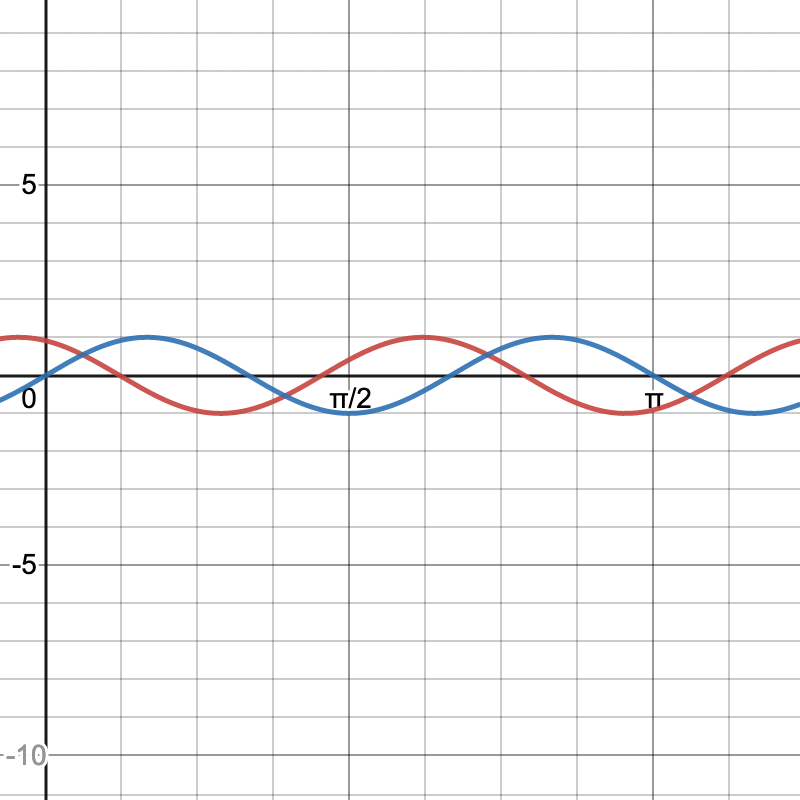
\includegraphics[width=0.5\textwidth]{figures/sine-wave-phase-shift.png}
	\caption{The phase shift in a sine wave}
	\label{fig:sine-wave-phase-shift}
\end{figure}

These three changes to an audio waveform will be the basis for the modules created in this project, in which some combination of modifications made to the audio signal will produce the desired changes. 